\section{214 --- Shortest Palindrome}
Given a string $s$, you are allowed to convert it to a palindrome by adding characters in front of it. Find and return the shortest palindrome you can find by performing this transformation.
\paragraph{Example 1:}
\begin{flushleft}
\textbf{Input}: \texttt{aacecaaa}
\\
\textbf{Output}: \texttt{aaacecaaa}
\end{flushleft}
\paragraph{Example 2:}
\begin{flushleft}
\textbf{Input}: \texttt{abcd}
\\
\textbf{Output}: \texttt{dcbabcd}
\end{flushleft}
\subsection{KMP}
由于只能在$s$的最前面插入字符,因此首先找到从$s[0]$开始最长的palindrome substring,假设其长度为$x$,即$s[0,x-1]$是palindrome。然后copy $s[x,l-1]$($l$是$s$的长度)到$y$,对$y$进行反转,然后$y+s$就是所求的最小长度的palindrome了。
\par
例如,$s=\texttt{abcbabcab}$. 从$s[0]$开始最长的palindrome substring 是\texttt{abcba}, 而剩下的部分是\texttt{bcab},其反转后为\texttt{bacb}. 因此,产生的最小长度palindrome即为$\texttt{bacb} + s = \texttt{bacbabcbabcab}$
\par
普通的方法所产生的时间复杂度为$O(n^2)$。因此需要KMP来进行优化。

\subsubsection{KMP Overview}
\textbf{KMP} is a string matching algorithm that runs in $O(n+m)$ times, where $n$ and $m$ are sizes of the text and string to be searched respectively. The key component of \textbf{KMP} is the failure function lookup table, say $f(s)$. The purpose of the lookup table is to store the length of the proper prefix of the string $b_{1}b_{2}\ldots b_{s}$ that is also a suffix of $b_{1}b_{2}\ldots b_{s}$
\par
This table is important because if we are trying to match a text string for $b_{1}b_{2}\ldots b_{n}$ and we have matched the first $s$ positions, but when we fail, then the value of lookup table for $s$ is the longest prefix of $b_{1}b_{2}\ldots b_{n}$ that could possibly match the text string up to the point we are at. Thus, we don't need to start all over again, and can resume searching from the matching prefix.
\par
The algorithm to generate the lookup table is easy and inutitive, as given below:
\setcounter{algorithm}{0}
\begin{algorithm}[H]
\caption{KMP Lookup Table Generation}
\begin{algorithmic}[1]
\Procedure{KMPTable}{$b, n$}
\State $\star$ Initialize an array $f$ with length $n$
\State $f[0]\gets 0$
\For{$i:=1 \to n-1$}
\State $t:=f[i-1]$
\While{$t > 0$ \textbf{and} $b[i]\neq b[t]$}
\State $t\gets f[t-1]$
\EndWhile
\If{$b[i]=b[t]$}
\State $t\gets t+1$
\EndIf
\State $f[i]\gets t$
\EndFor
\EndProcedure
\end{algorithmic}
\end{algorithm}
\begin{itemize}
\item First set $f(0)=0$ since no proper prefix is available.
\item Next, iterate over $i$ from $1$ to $n-1$:
\begin{itemize}
\item Set $t=f(i-1)$
\item While $t>0$ and letter at $i$ doesn't match the letter at $t$ position, set $t=f(t)$, which essentially means that we have problem matching and must consider a shorter prefix, which will be $b_{f(t-1)}$, until we find a match or t becomes 0.
\item If $b[i]=b[t]$, increments $t$ 
\item Set $f[i]\gets t$
\end{itemize}
\end{itemize}
The lookup table generation is as illustrated below:
\par
Take a string \texttt{cacacabc} as an example:
\par
At start No proper prefix $f[0]=0$
\begin{figure}[H]
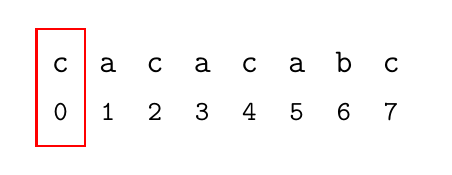
\begin{tikzpicture}
\matrix(m)[nodes={minimum size=6mm}, column sep= 0mm, anchor=base]
{
\node(1){\large \texttt{c}}; & \node(2){\large \texttt{a}};
& \node(3){\large \texttt{c}};& \node(4){\large \texttt{a}};
& \node(5){\large \texttt{c}};& \node(6){\large \texttt{a}};
& \node(7){\large \texttt{b}};& \node(8){\large \texttt{c}};\\
\node(21){\texttt{0}}; & \node(22){\texttt{1}};
& \node(23){\texttt{2}};& \node(24){\texttt{3}};
& \node(25){\texttt{4}};& \node(26){\texttt{5}};
& \node(27){\texttt{6}};& \node(28){\texttt{7}};\\
};
\draw[red, line width=0.3mm] (m.north west -| 1.west) rectangle (m.south west -| 1.east);
\end{tikzpicture}
\end{figure}
\begin{enumerate}
\item $i=1$, $t\gets f[0]$ so $t=0$
\begin{figure}[H]
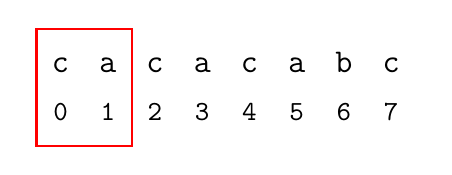
\begin{tikzpicture}
\matrix(m)[nodes={minimum size=6mm}, column sep= 0mm, anchor=base]
{
\node(1){\large \texttt{c}}; & \node(2){\large \texttt{a}};
& \node(3){\large \texttt{c}};& \node(4){\large \texttt{a}};
& \node(5){\large \texttt{c}};& \node(6){\large \texttt{a}};
& \node(7){\large \texttt{b}};& \node(8){\large \texttt{c}};\\
\node(21){\texttt{0}}; & \node(22){\texttt{1}};
& \node(23){\texttt{2}};& \node(24){\texttt{3}};
& \node(25){\texttt{4}};& \node(26){\texttt{5}};
& \node(27){\texttt{6}};& \node(28){\texttt{7}};\\
};
\draw[red, line width=0.3mm] (m.north west -| 1.west) rectangle (m.south west -| 2.east);
\end{tikzpicture}
\end{figure}
No proper prefix equal to suffix yet. Therefore $f[1] \gets 0$.
\item $i=2$, $t\gets f[1]$ so $t=0$, but $b[2] = b[0] = c \Longrightarrow t\gets t+1$
\begin{figure}[H]
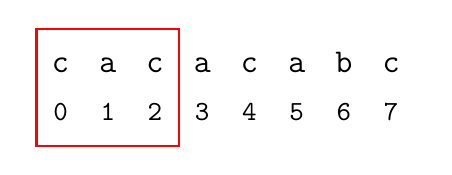
\begin{tikzpicture}
\matrix(m)[nodes={minimum size=6mm}, column sep= 0mm, anchor=base]
{
\node(1){\large \texttt{c}}; & \node(2){\large \texttt{a}};
& \node(3){\large \texttt{c}};& \node(4){\large \texttt{a}};
& \node(5){\large \texttt{c}};& \node(6){\large \texttt{a}};
& \node(7){\large \texttt{b}};& \node(8){\large \texttt{c}};\\
\node(21){\texttt{0}}; & \node(22){\texttt{1}};
& \node(23){\texttt{2}};& \node(24){\texttt{3}};
& \node(25){\texttt{4}};& \node(26){\texttt{5}};
& \node(27){\texttt{6}};& \node(28){\texttt{7}};\\
};
\draw[red, line width=0.3mm] (m.north west -| 1.west) rectangle (m.south west -| 3.east);
\end{tikzpicture}
\end{figure}
Suffix and prefix both are {\LARGE \texttt{c}}. Hence $f[2]\gets t=1$

\item $i=3$, $t\gets f[2]$ so $t=1$, but $b[3] = b[1] = a \Longrightarrow t\gets t+1$
\begin{figure}[H]
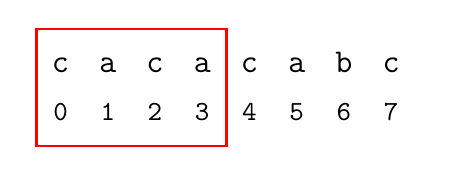
\begin{tikzpicture}
\matrix(m)[nodes={minimum size=6mm}, column sep= 0mm, anchor=base]
{
\node(1){\large \texttt{c}}; & \node(2){\large \texttt{a}};
& \node(3){\large \texttt{c}};& \node(4){\large \texttt{a}};
& \node(5){\large \texttt{c}};& \node(6){\large \texttt{a}};
& \node(7){\large \texttt{b}};& \node(8){\large \texttt{c}};\\
\node(21){\texttt{0}}; & \node(22){\texttt{1}};
& \node(23){\texttt{2}};& \node(24){\texttt{3}};
& \node(25){\texttt{4}};& \node(26){\texttt{5}};
& \node(27){\texttt{6}};& \node(28){\texttt{7}};\\
};
\draw[red, line width=0.3mm] (m.north west -| 1.west) rectangle (m.south west -| 4.east);
\end{tikzpicture}
\end{figure}
Suffix and prefix both are {\LARGE \texttt{ca}}. Hence $f[3]\gets t=2$

\item $i=4$, $t\gets f[3]$ so $t=2$, but $b[4] = b[2] = c \Longrightarrow t\gets t+1$,
\begin{figure}[H]
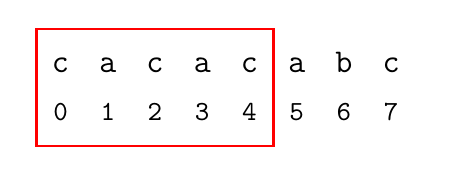
\begin{tikzpicture}
\matrix(m)[nodes={minimum size=6mm}, column sep= 0mm, anchor=base]
{
\node(1){\large \texttt{c}}; & \node(2){\large \texttt{a}};
& \node(3){\large \texttt{c}};& \node(4){\large \texttt{a}};
& \node(5){\large \texttt{c}};& \node(6){\large \texttt{a}};
& \node(7){\large \texttt{b}};& \node(8){\large \texttt{c}};\\
\node(21){\texttt{0}}; & \node(22){\texttt{1}};
& \node(23){\texttt{2}};& \node(24){\texttt{3}};
& \node(25){\texttt{4}};& \node(26){\texttt{5}};
& \node(27){\texttt{6}};& \node(28){\texttt{7}};\\
};
\draw[red, line width=0.3mm] (m.north west -| 1.west) rectangle (m.south west -| 5.east);
\end{tikzpicture}
\end{figure}
Suffix and prefix both are {\LARGE \texttt{cac}}. Hence $f[4]\gets t=3$

\item $i=5$, $t\gets f[4]$ so $t=3$, but $b[5] = b[3] = a \Longrightarrow t\gets t+1$,
\begin{figure}[H]
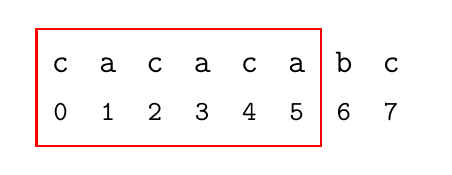
\begin{tikzpicture}
\matrix(m)[nodes={minimum size=6mm}, column sep= 0mm, anchor=base]
{
\node(1){\large \texttt{c}}; & \node(2){\large \texttt{a}};
& \node(3){\large \texttt{c}};& \node(4){\large \texttt{a}};
& \node(5){\large \texttt{c}};& \node(6){\large \texttt{a}};
& \node(7){\large \texttt{b}};& \node(8){\large \texttt{c}};\\
\node(21){\texttt{0}}; & \node(22){\texttt{1}};
& \node(23){\texttt{2}};& \node(24){\texttt{3}};
& \node(25){\texttt{4}};& \node(26){\texttt{5}};
& \node(27){\texttt{6}};& \node(28){\texttt{7}};\\
};
\draw[red, line width=0.3mm] (m.north west -| 1.west) rectangle (m.south west -| 6.east);
\end{tikzpicture}
\end{figure}
Suffix and prefix both are {\LARGE \texttt{caca}}. Hence $f[5]\gets t=4$

\item $i=6$, $t=f[5]$ so $t=4$, now $b[6]\neq b[4] \Longrightarrow t\gets f[t-1]$ which leads to $t\gets f[3]=2$. However, $b[6]\neq b[2] \Longleftrightarrow t\gets f[t-1]$ which further leads to $t\gets f[1]$. Now $t$ is updated to zero.
\begin{figure}[H]
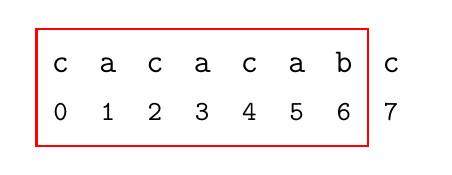
\begin{tikzpicture}
\matrix(m)[nodes={minimum size=6mm}, column sep= 0mm, anchor=base]
{
\node(1){\large \texttt{c}}; & \node(2){\large \texttt{a}};
& \node(3){\large \texttt{c}};& \node(4){\large \texttt{a}};
& \node(5){\large \texttt{c}};& \node(6){\large \texttt{a}};
& \node(7){\large \texttt{b}};& \node(8){\large \texttt{c}};\\
\node(21){\texttt{0}}; & \node(22){\texttt{1}};
& \node(23){\texttt{2}};& \node(24){\texttt{3}};
& \node(25){\texttt{4}};& \node(26){\texttt{5}};
& \node(27){\texttt{6}};& \node(28){\texttt{7}};\\
};
\draw[red, line width=0.3mm] (m.north west -| 1.west) rectangle (m.south west -| 7.east);
\end{tikzpicture}
\end{figure}
No proper prefix equal to suffix. Hence $f[6]\gets t=0$

\item $i=7$, $t=f[6]$ so $t=0$, but $b[7] = b[0]\Longrightarrow t\gets t+1$
\begin{figure}[H]
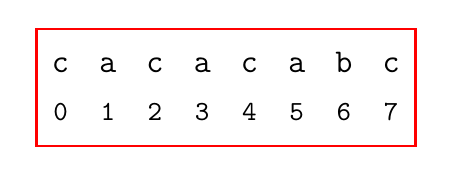
\begin{tikzpicture}
\matrix(m)[nodes={minimum size=6mm}, column sep= 0mm, anchor=base]
{
\node(1){\large \texttt{c}}; & \node(2){\large \texttt{a}};
& \node(3){\large \texttt{c}};& \node(4){\large \texttt{a}};
& \node(5){\large \texttt{c}};& \node(6){\large \texttt{a}};
& \node(7){\large \texttt{b}};& \node(8){\large \texttt{c}};\\
\node(21){\texttt{0}}; & \node(22){\texttt{1}};
& \node(23){\texttt{2}};& \node(24){\texttt{3}};
& \node(25){\texttt{4}};& \node(26){\texttt{5}};
& \node(27){\texttt{6}};& \node(28){\texttt{7}};\\
};
\draw[red, line width=0.3mm] (m.north west -| 1.west) rectangle (m.south west -| 8.east);
\end{tikzpicture}
\end{figure}
Suffix and prefix both are {\LARGE \texttt{c}}. Hence $f[7]\gets t=1$
\end{enumerate}
The final table is:
\begin{table}[H]
\begin{tabular}{|c|l|l|l|l|l|l|l|l|}
\hline
$i$    & 0 & 1 & 2 & 3 & 4 & 5 & 6 & 7 \\ \hline
$f(i)$ & 0 & 0 & 1 & 2 & 3 & 4 & 0 & 1 \\ \hline
\end{tabular}
\end{table}

\subsubsection{Apply KMP}
如果把$s$进行反转,然后append在$s$后,这样问题就转变成求最长的proper prefix which is equal to suffix。这样就需要KMP lookup table了。
\begin{itemize}
\item 将$s$ reverse 为 $\hat{s}$
\item 在$s$和$\hat{s}$中间加入一个特殊字符 t, 比如\$。形成一个新的string $x$,即$x=s+t+\hat{s}$。这个$t$是必须的,比如\texttt{aaaa},如果不加$t$,$x=\texttt{aaaaaaaa}$,那么最长的prefix就是\texttt{aaaaaaa},长度为7。(注意,prefix是不包含整个string的)。
\item 生成$x$的KMP lookup table $f$。那么$f[l_t-1]$的长度就是$t$最长的prefix与suffix相等的substring的长度。于是$s$中反转的部分即为$\hat{s}[0, l_s-f[l_t-1]$
\item $\hat{s}[0, l_s-f[l_t-1]] + s$即为所能生成的最小长度的palindrome string。
\end{itemize}
\setcounter{lstlisting}{0}
\begin{lstlisting}[style=customc, caption={KMP Table}]
string shortestPalindrome( string s )
{
    string r;
    r = s;

	//reverse s
    reverse( r.begin(), r.end() );

    string x;
    //reserve x memory to avoid memory allocation
    x.reserve( s.size() + r.size() + 1 );

    x = s;
    x.push_back( '*' );
    x += r;

	//Generate KMP table
    vector<int> f( x.size(), 0 );

    for( size_t i = 1; i < x.size(); ++i )
    {
        int t = f[i - 1];

        while( ( t > 0 ) && ( x[t] != x[i] ) )
        {
            t = f[t - 1];
        }

        if( x[t] == x[i] )
        {
            ++t;
        }

        f[i] = t;
    }
    string ans = r.substr( 0, s.size() - f.back() );
    ans += s;
    return ans;
}
\end{lstlisting}
